\documentclass[a4paper,14pt]{extarticle}
\usepackage[left=2.5cm, right=1.5cm, vmargin=2.5cm]{geometry}
\usepackage[utf8]{inputenc}
\usepackage[T2A]{fontenc}
\usepackage[russian]{babel}
\usepackage{graphicx}
\graphicspath{{pictures/}}
\usepackage{caption}
\usepackage{subcaption}
\usepackage{indentfirst}
\setlength\parindent{5ex}
\usepackage{fancyhdr}
\usepackage{booktabs}
\usepackage{siunitx} 
\usepackage{pgfplotstable}
\usepackage{amsmath}
\usepackage{autonum}
\usepackage{amsfonts}
\DeclareMathOperator{\sign}{sgn}
\newcommand{\gt}{\textgreater} % знак больше
\newcommand{\lt}{\textless}       % знак меньше
\DeclareGraphicsExtensions{.pdf,.png,.jpg}
\pagestyle{fancy}
\fancyhf{}
\rhead{\thepage}
\renewcommand{\headrulewidth}{0pt}

\fancypagestyle{plain}{ 
	\fancyhf{}
	\rhead{\thepage}}

\author{Никитин Илья}

\title{Отчет по лабораторной работе №2: "Гистерезис"}
\date{\today}

\begin{document}
	
	\maketitle
	\tableofcontents
	
	\section{Оборудование}
		\begin{itemize}
			\item Цифровой осциллограф Rigol со встроенным генератором синусоидального напряжения
			\item ЛАТР
			\item Понижающий трансформатор
			\item Клемник для сборки электрических цепей
			\item Ферритовый сердечник
			\item Резистор с сопротивлением 100 мОм
			\item Резистор с сопротивлением 95 Ом
			\item Резистор с сопротивлением 792 кОм
			\item Конденсатор емкостью около 1 мкФ
			\item Толстая медная проволока
		\end{itemize}
	\section{Задачи}
		\begin{itemize}
			\item Изготовить катушку индуктивности с ферритовым сердечником и измерить ее
			индуктивность
			\item Пронаблюдать петлю магнитного гистерезиса и измерить магнитные параметры материала сердечника: зависимость намагниченности и магнитной восприимчивости образца от поля, коэрцитивную силу и остаточную намагниченность.
		\end{itemize}
	\section{Определение индуктивности катушки}
		\subsection{Теория работы}
			\begin{figure}[h]
				\centering
				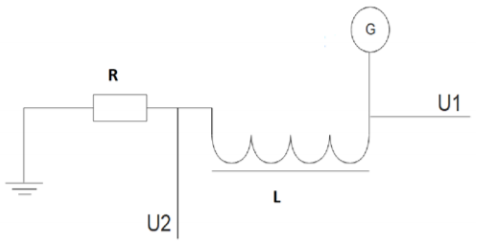
\includegraphics[width=.75\linewidth]{схема.png}
				\caption{Схема измерения индуктивности. $R$ – резистор сопротивлением 95 Ом, $L$ – катушка, индуктивность которой требуется измерить, $G$ – выход встроенного	генератора осциллографа, $U_1$ и $U_2$ – напряжения, измеряемое на первом и втором каналах осциллографа. Земля у генератора и обоих входов осциллографа общая.}
				\label{fig1}
			\end{figure}
			\newpage
			С генератора подается синусоидальный сигнал с амплитудой 12 В. В приближении, что резистор имеет только активное сопротивление, а катушка только реактивное можно рассчитать импеданс катушки $Z_L = i \omega L$ зная $U_1$, $U_2$ и $R$. Полный импеданс всей цепи равен $Z_\Sigma =	R + i \omega L$. Тогда модули (и амплитуды) тока и напряжения в цепи связаны следующим образом: $U_0 = I_0 \sqrt{R^2 + (\omega L)^2}$. Также из этого легко найти модуль тангенса разности фаз между током и напряжением: $tan(\phi) = \frac{\omega L}{R}$. Измеряемое напряжение $U_2$ равно произведению величины тока в цепи на сопротивление $R$, из это получим связь между $U_1$ и $U_2$: $\frac{U_1}{U_2} = \sqrt{1 + (\frac{\omega L}{R})^2}$, из которой можно найти индуктивность $L$. Из этого соотношения легко понять требования на величину сопротивления $R$ и частоту $\omega$: они должны быть такими, чтобы величина $\frac{\omega L}{R}$ заметно превышала единицу, иначе измерения будут неточными.
		\subsection{Ход работы}
			В первую очередь требовалось сделать катушку — намотать медную проволоку на
			ферритовый сердечник. Мы взяли уже намотанную катушку, измерили ее геометрические размеры. Катушка была намотана из толстой медной проволоки и состояла из 42 витков.
			Далее была собрана схема (\ref{fig1}). С помощью осциллографа были измерены напряжения на катушке для токов на различных частотах, затем определены различные значения выражения $\frac{R}{2\pi}\sqrt{(\frac{U_1}{U_2})^2 - 1}$ при различных значениях частоты.
		\subsection{Обработка данных}
			По полученным точкам были построены прямые по МНК и взвешенному МНК, коэффициентом которых является искомая индуктивность катушки.
			\begin{figure}[h]
				\centering
				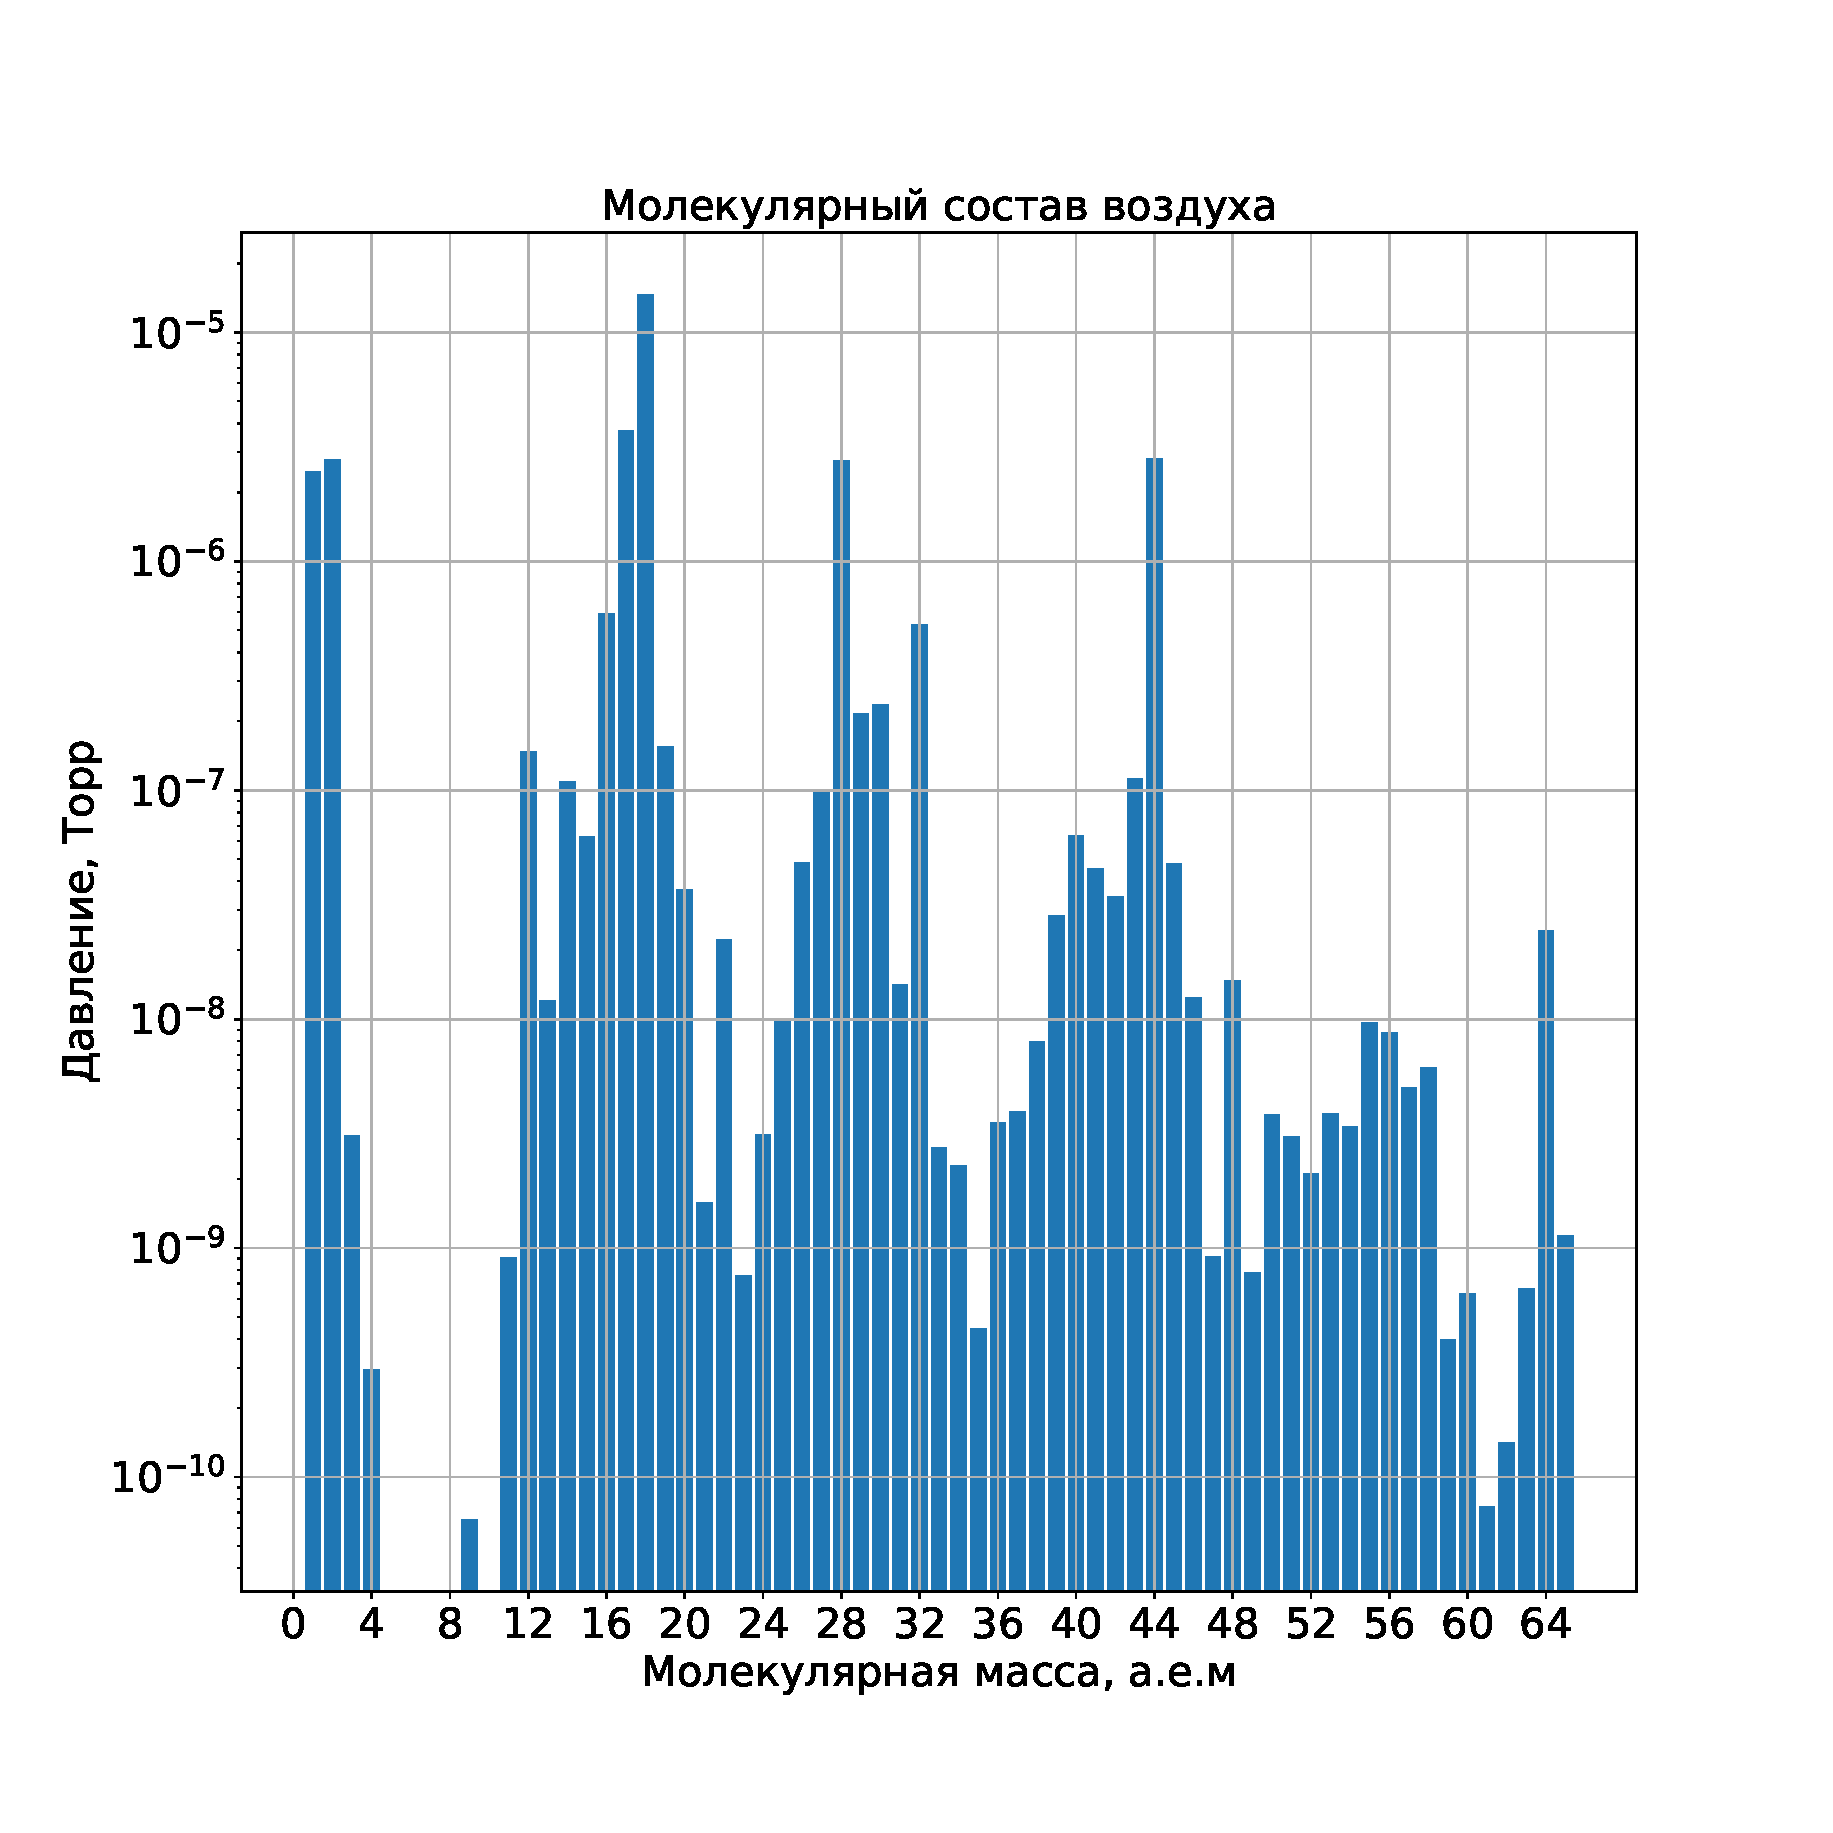
\includegraphics[width=.80\linewidth]{Lab2_1.eps}
				\caption{На графике изображены две прямые: прямая, построенная по экспериментальным данным с помощью МНК и прямая, построенная с помощью взвешенного МНК}
				\label{fig2}
			\end{figure} 
			\newpage
			За основу был взят график, построенный по взвешенному МНК, так как при предыдущих измерениях индуктивности катушки получившийся результат лучше соотносился с заявленной индуктивностью и показателями точных приборов. Получившаяся индуктивность с учетом погрешностей:
			\begin{equation}
				L = 2.73 \pm 0.10\text{мГн}
			\end{equation}
	\section{Гистерезис}
		\subsection{Теория работы}
			Для получения картины магнитного гистерезиса необходимо собрать одну из следующих схем:
			\begin{figure}[h]
				\centering
				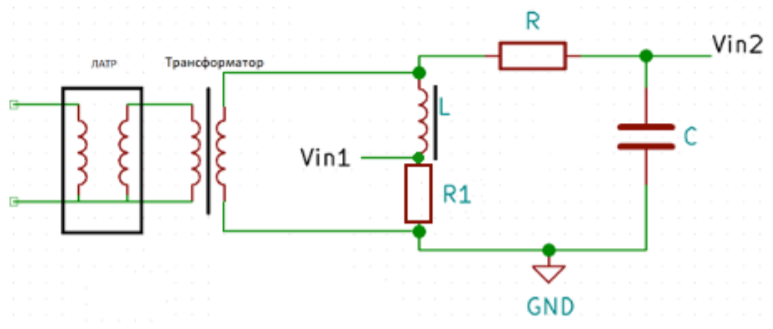
\includegraphics[width=0.9\linewidth]{схема2.png}
				\caption{Схема измерительной цепи с одной катушкой}
				\label{fig3}
			\end{figure}
			\newline
			\begin{figure}[h]
				\centering
				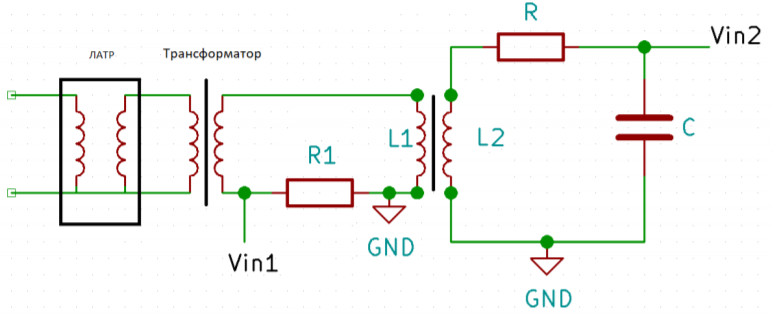
\includegraphics[width=0.9\linewidth]{схема3.png}
				\caption{Схема измерительной цепи с двумя катушками}
				\label{fig3}
			\end{figure}
			\newpage
			Принципиально схемы отличаются мало. В обеих ЛАТР (лабораторный автотрансформатор) используется для питания схемы от сети и регулировки силы тока. Понижающий трансформатор нужен для повышения выходного тока и гальванической развязки схемы от сети. Резистор $R_1$ малого сопротивления ($0.1-1$ Ом) необходим для измерения силы тока, текущего через катушку, $L (L1)$ – собственно катушка из медной проволоки, намотанная на образец. Сопротивление $R$ (номиналом $240 - 800$ кОм) и	конденсатор $С$ (емкостью в несколько микрофарад) образуют интегрирующую напряжение на катушке цепочку. Напряжение ${\text{Vin}}_1$, пропорциональное току через катушку и, соответственно, напряженности поля $H$ в ней, и напряжение ${\text{Vin}}_2$, пропорциональное интегралу напряжения на катушке и, следовательно потоку и индукции поля B через нее, подаются на два канала осциллографа. 
			Далее, настроив коэффициенты усиления каналов осциллографа и напряжение на входе ЛАТРа можно получить на экране осциллографа изображение петли гистерезиса. Это изображение можно записать (например, на flesh накопитель) и перерисовать в координатах B(H), получив в результате картину магнитного гистерезиса в образце. Cвязь напряженности поля H и тока в цепи I находится по теореме о циркуляции: $\oint\limits\mathbf{H}\cdot d\mathbf{l} = I$, откуда $H = \frac{N_1 I}{\pi D}$, где N1 – число витков в первой катушке, D – средний диаметр тороидального сердечника.
			Связан с напряжением $\text{Vin}_1$ по закону Ома: $\text{Vin}_1 = R_1 I$. Напряжение на катушке (первой или второй) по закону Фарадея пропорционально производной индукции поля B в сердечнике: $V = -\frac{d\Phi}{dt} = -SN_i\frac{dB}{dt}$. Здесь $S$ – площадь поперечного сечения тороидального сердечника, $N_i$ - число витков в катушке. Для того чтобы	измерять сигнал пропорциональный индукции поля используется интегрирующая цепочка из сопротивления $R$ емкости $С$. Можно показать, что если постоянная времени цепочки $RC$ значительно превышает период изменения сигнала (в данном случае это период колебания напряжения в сети электроснабжения равный 17 мс), то напряжение на конденсаторе $\text{Vin}_2$	равно $\frac{1}{RC}\int V dt = \frac{1}{RC}S N_1 B$. Тогда напряжение $\text{Vin}_2$ пропорционально индукции поля в образце.
		\subsection{Ход работы}
			В ходе работы были собраны обе схемы. Для второй схемы потребовалось намотать на исходную катушку вторую катушку из 56 витков. Провода для нее использовались тонкие, так как по данной катушке текли небольшие токи. Данные снимались с помощью цифрового осциллографа для дальнейшего анализа.
		\subsection{Анализ данных}
			\subsubsection{Первая схема}
				Для первой схемы был получен один график петли гистерезиса, так как уже на малых напряжениях картина получалась искаженной. 
				\begin{figure}[h!]
					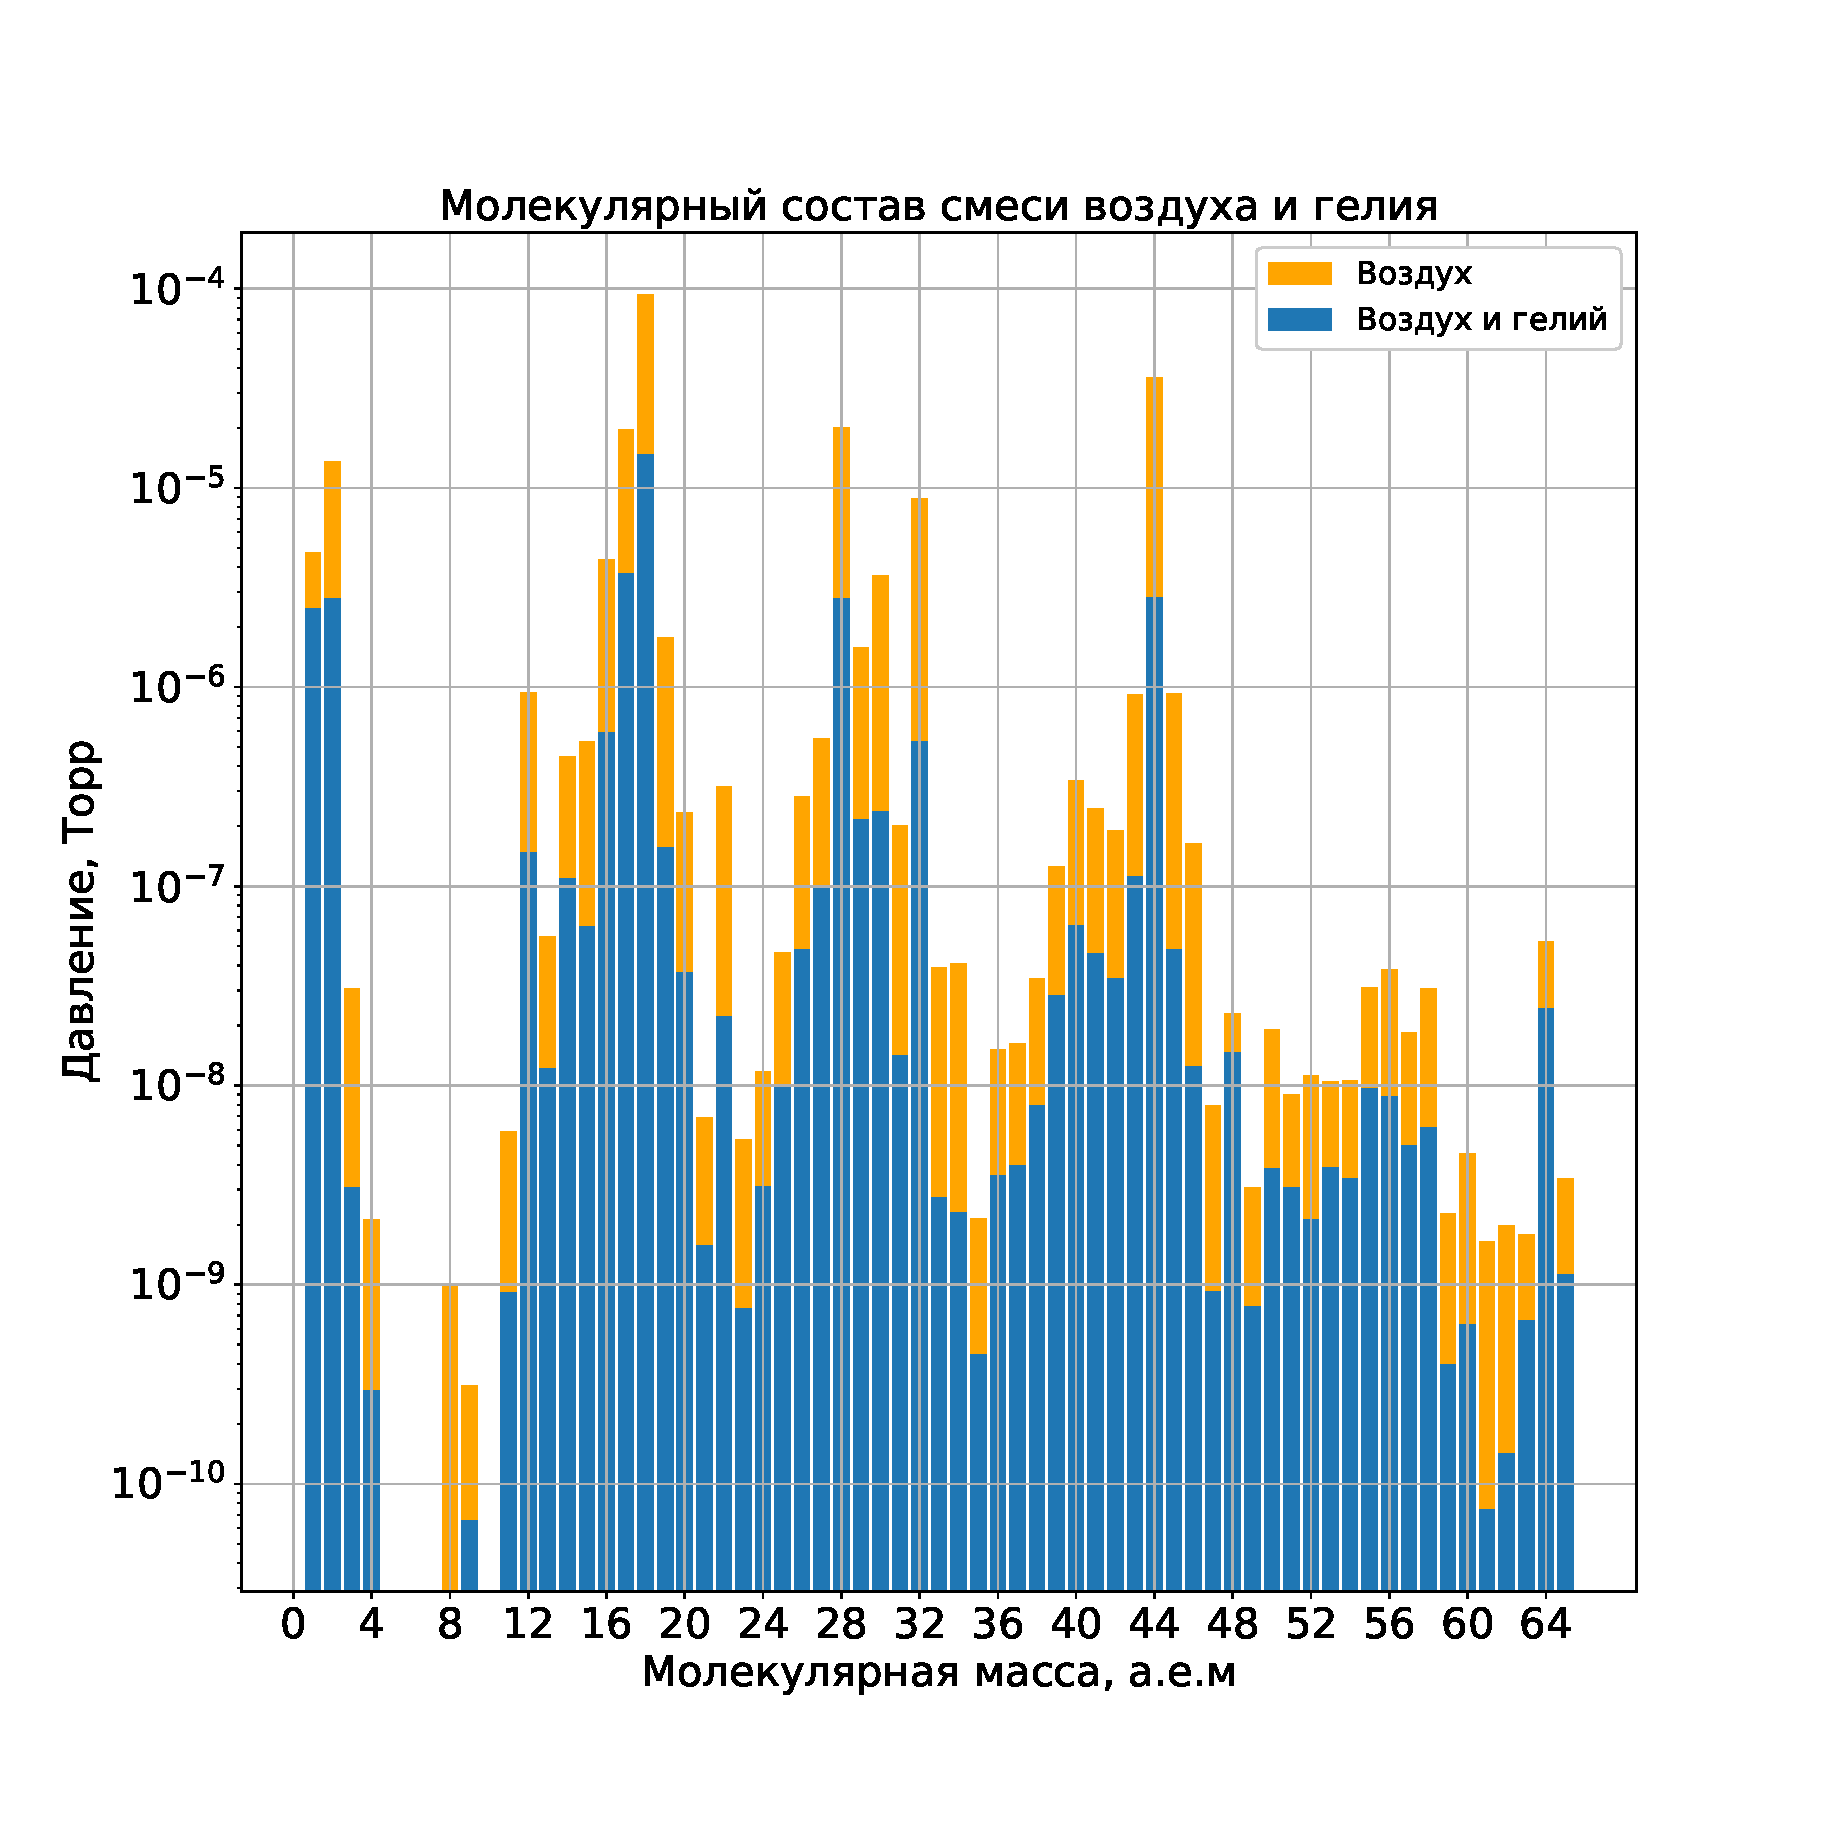
\includegraphics[width=1.0\linewidth]{Lab2_3.eps}
					\caption{4 проводная схема измерения малого сопротивления}
					\label{fig5}
				\end{figure}
				\newline
			\subsubsection{Ход работы}
				В ходе работы с помощью мультиметра и блока питания с амперметром были измерены показания напряжения на образце в зависимости от заданной силы тока на блоке питания.
				\begin{figure}[h]
					\centering
					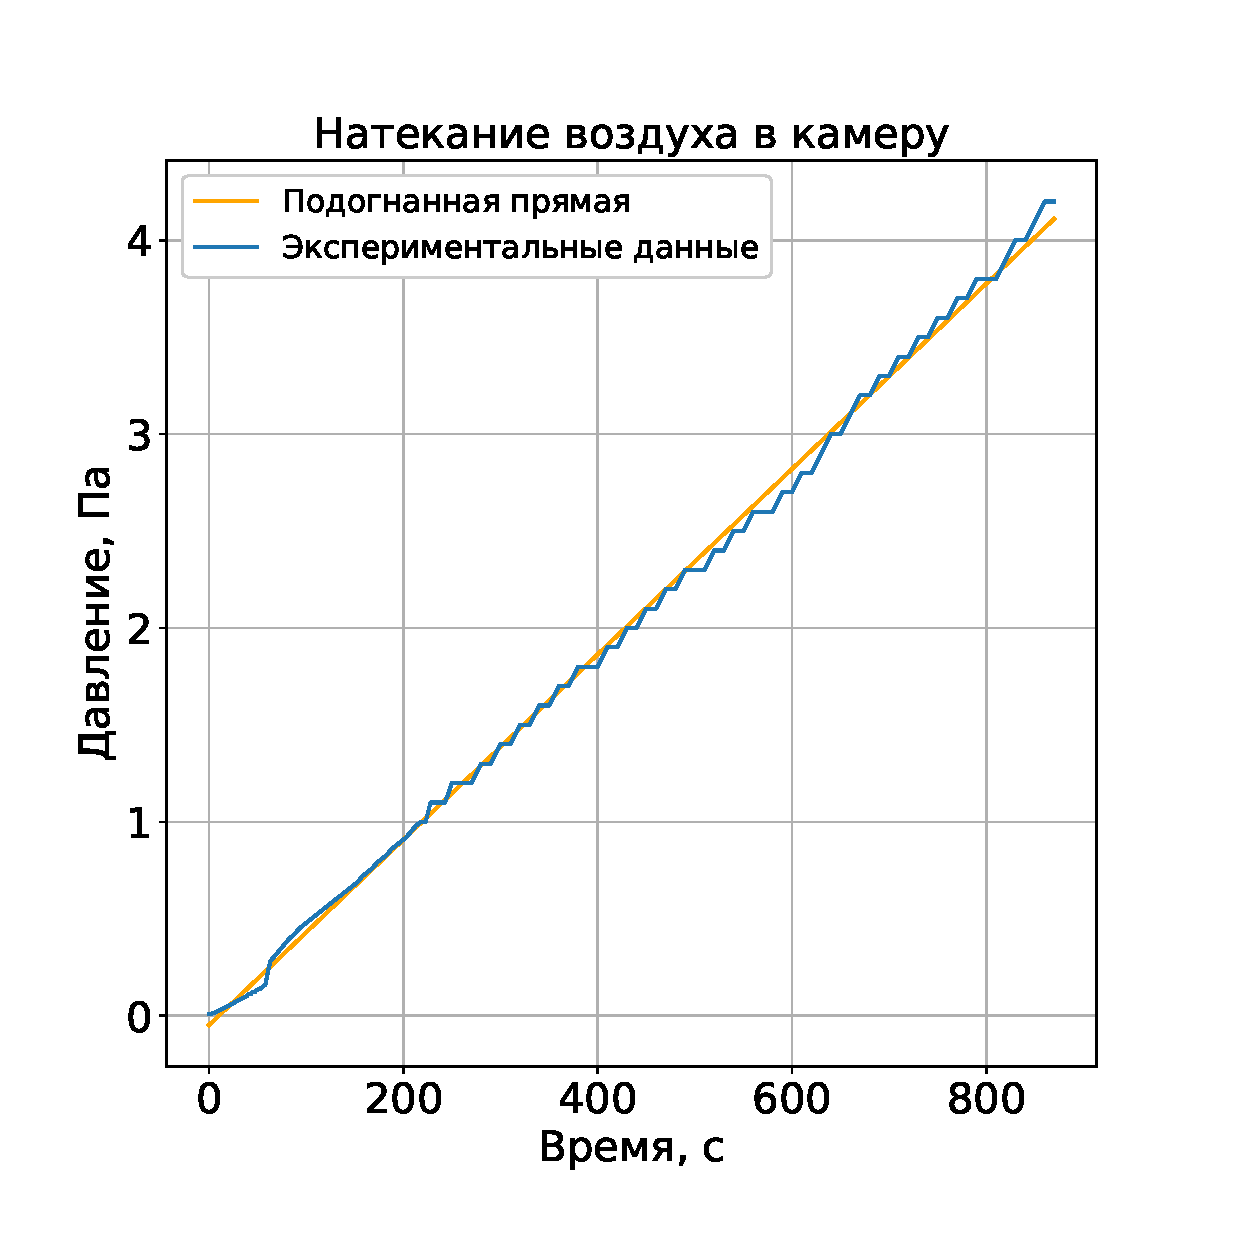
\includegraphics[width=.80\linewidth]{Lab1_3.eps}
					\caption{Зависимость напряжения от тока на образце}
					\label{fig6}
				\end{figure}
				\newpage
				С помощью была МНК построена прямая, коэффициент которой определяет искомое значение сопротивления образца $R = 4.1 \pm 0.1$ КОм
	\section{Генератор Ван Дер Граафа}
		\subsection{Оборудование}
			\begin{itemize}
				\item Генератор Ван де Граафа 
				\item Источник постоянного тока для питания
				электродвигателя 
				\item Осциллограф 
				\item Щуп для осциллографа – 1 шт. 
				\item Мультиметр 
				\item Высоковольтный кабель для подключения к сфере генератора 
				\item Провода для заземления
			\end{itemize}
		\subsection{Задачи}
			\begin{itemize}
				\item Определить напряжение пробоя воздуха  
				\item Определить напряжение генератора Ван Дер Граафа по длине газового разряда в воздухе
			\end{itemize}
		\subsection{Измерение тока генератора}	
			\subsubsection{Теория работы}
				Измерить ток генератора $I$. Для этого подключить к генератору мультиметр. Напряжение на генераторе задается источником питания. Провести измерения при различных скоростях вращения ленты (задается установкой напряжения на источнике питания).
				\begin{figure}[h]
					\centering
					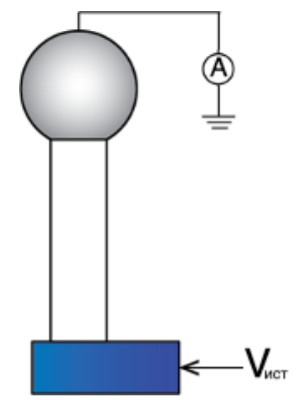
\includegraphics[width=.30\linewidth]{Схема4.png}
					\caption{Схема измерения тока генератора}
					\label{fig7}
				\end{figure}
				\newpage
			\subsubsection{Ход работы}
				В ходе работы к генератору был подключен мультиметр, ток был измерен при разных напряжениях, подаваемых генератором.
				\begin{figure}[h]
					\centering
					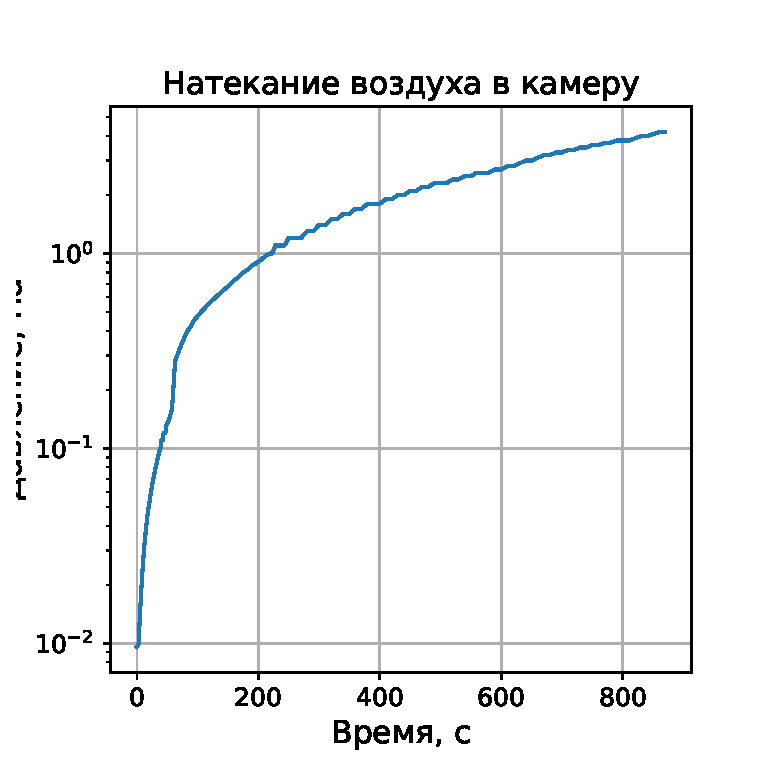
\includegraphics[width=.80\linewidth]{Lab1_4.eps}
					\caption{Зависимость напряжения от тока на генераторе}
					\label{fig8}
				\end{figure}
				\newpage
				С помощью МНК была построена прямая, определяющая коэффициент пропорциональности (сопротивление): $U = 1.132 I + 2.393$
		\subsection{Определение напряжения пробоя воздуха}
			\subsubsection{Теория работы}
				Вернуть обратно малую заземленную сферу. Измерить период искрового разряда $T$ при помощи осциллографа. Для измерения достаточно расположить осциллограф	недалеко от генератора, период наводок на экране осциллографа совпадает с периодами искрового разряда. Следует избегать прямого подключения любых измерительных приборов к высоковольтному генератору. 
				\newline
				Пренебрегая ёмкостью малой сферы, оценить ёмкость большой сферы генератора как $C = 4 \pi \epsilon_0 r$ где $r$ – радиус сферы. 
				\newline
				Измерить период искрового разряда $T$ для различных расстояний между сферами.
				\newline 
				Полученные выше измерения позволяют оценить напряжение пробоя в зависимости от расстояния $d$ между сферами:
				$E_{bd} = \frac{IT}{dC}$
				\newline
				Оценить погрешность измерений.
			\subsubsection{Ход работы}
				В ходе работы были измерены периоды искрового разряда $T$ для разных расстояний при 2 сериях напряжений.
				\begin{figure}[h]
					\centering
				 	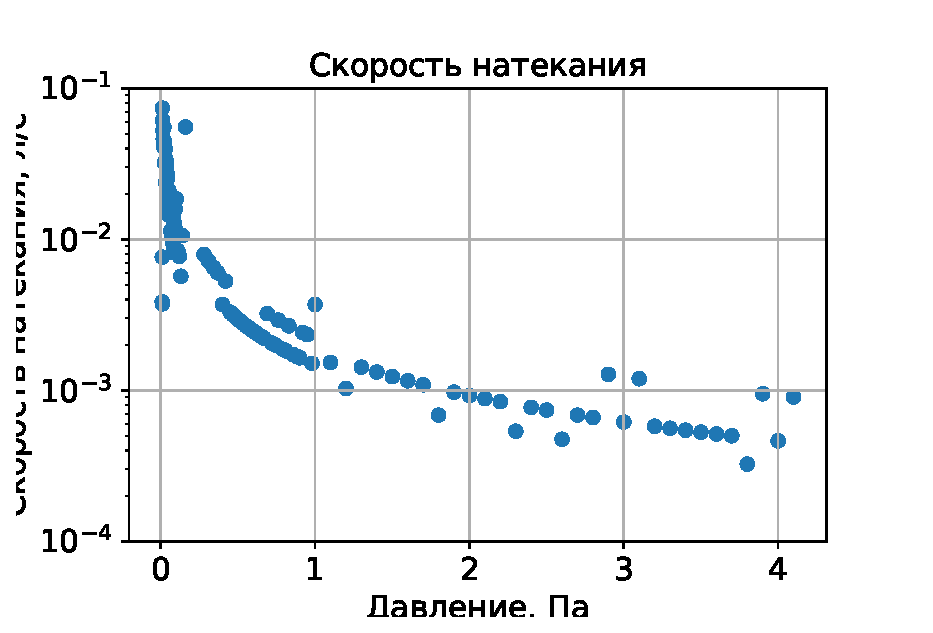
\includegraphics[width=.80\linewidth]{Lab1_5.eps}
				 	\caption{Зависимость напряжения пробоя воздуха от расстояния между сферами}
				 	\label{fig9}
				\end{figure}
				\newpage
				С помощью МНК была построена прямая, коэффициентом которой является напряженность пробоя воздуха $E_{bd} = 23 \pm 3$ кВ/см
		\subsection{Оценка напряжений генератора}
			\subsubsection{Теория работы}
				Один из способов измерения больших напряжений – шаровые измерительные разрядники. Порядок измерений высоковольтных напряжений регламентируются в ГОСТ 17512-82 [1]. Напряжение пробоя газов сильно зависит от давления, состава газа и формы
				электродов. Пренебрегая тем, что сферы имеют различный диаметр, определить напряжение генератора для различных скоростей вращения ленты. Для различных расстояний между сферами $d$ определить напряжение по Таблице 1. Для условий отличающихся от нормальных следует использовать поправочный
				коэффициент $k: U_{tr} = k U_{tab}$, где $U_{tab}$– значение разрядного напряжения определенное из Таблицы 1, $U_tr$ - истинное значение напряжения. Для значений относительной плотности воздуха от 0.95 до 1.05 поправочный коэффициент $k$ можно оценить как: $k = 0.386 \frac{P}{273+t}$где давление $P$ выражено в миллиметрах ртутного столба, а температура $t$ в градусах Цельсия.
				\newline
				Сравнить полученные результаты с результатами из первой части работы.
			\subsubsection{Ход работы}
				В ходе работы на графике из предыдущей части была построена зависимость напряжения от расстояния предлагаемая Таблицой 1
				\begin{figure}[h!]
					\centering
					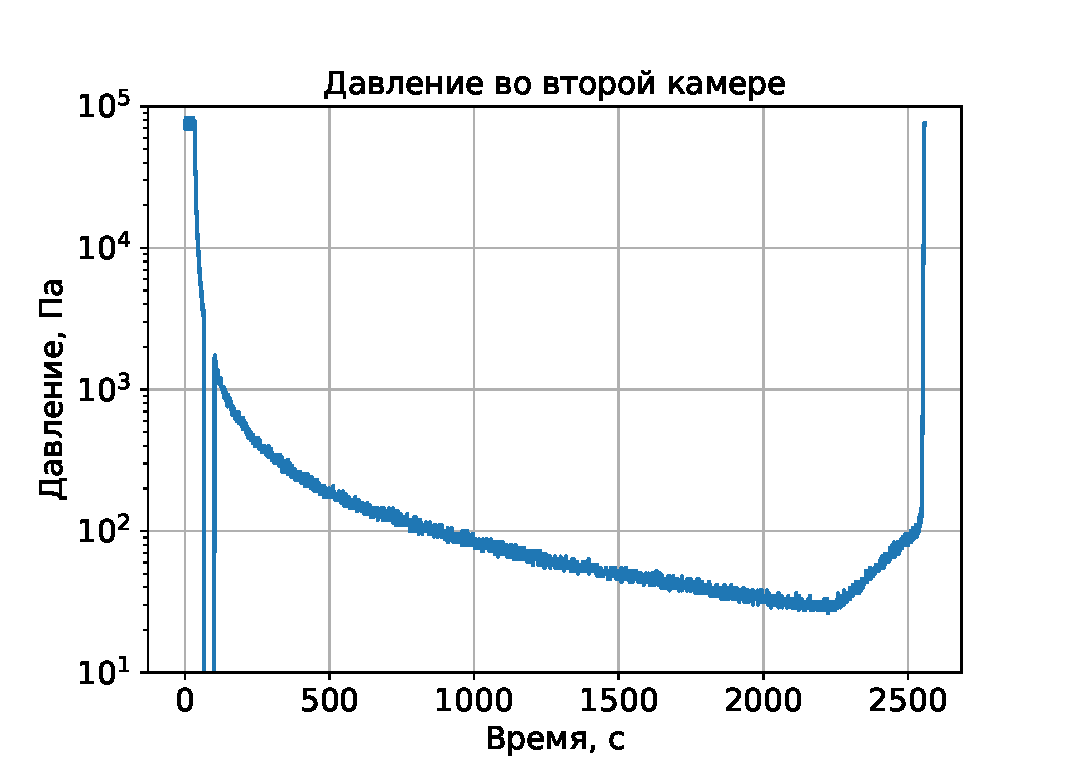
\includegraphics[width=.80\linewidth]{Lab1_6.eps}
					\caption{Зависимость напряжения пробоя воздуха от расстояния между сферами}
					\label{fig10}
				\end{figure}
				\newline
				На график добавилась прямая черного цвета, она соответствует зависимости, построенной по данным из Таблицы 1. Ее коэффициент наклона равен напряженности пробоя воздуха $E_{bd} = 26$ Кв/м. Как можно заметить, коэффициены прямых отличаются, но в пределах погрешности экспериментальных данных.
\end{document}